\documentclass[a4paper,12pt]{article}
\usepackage[utf8]{inputenc}
\usepackage[T1]{fontenc}
\usepackage[italian]{babel}
\usepackage{graphicx}
\usepackage{hyperref}
\usepackage{geometry}
\usepackage{float}
\usepackage{listings}
\usepackage{xcolor}

\geometry{margin=2.5cm}
\setlength{\parindent}{0pt}
\setlength{\parskip}{1em}

\title{\textbf{S.I.S.I.F.O.: Progettazione e Realizzazione di un Sistema Autonomo di Mini-Golf}}
\author{Laboratorio di Making}
\date{dicembre 2025}

\begin{document}

\maketitle

\begin{abstract}
Questa relazione documenta il processo di sviluppo, costruzione e debugging di "S.I.S.I.F.O.", un robot autonomo progettato per giocare a mini-golf su una piattaforma integrata.\\
Il progetto integra visione artificiale, pianificazione dei tiri tramite Large Language Model (LLM) e un sistema hardware non triviale.\\
Speciale attenzione viene data alle sfide costruttive artigianali, alle problematiche elettroniche riscontrate e alle soluzioni pratiche adottate per il progetto.
\end{abstract}

\tableofcontents
\newpage

\section{Introduzione}
L'obiettivo del progetto era creare un sistema in grado di percepire l'ambiente di gioco, decidere una strategia di tiro e attuarla fisicamente.

La mia inesperienza ha messo tanti bastoni tra le mie ruote, e forse il progetto era alquanto ambizioso per la consegna, ma sono riuscito a venire a patto con la visione che avevo.

Il risultato è un robot costruito con materiali di recupero e componenti elettronici avanzati (Raspberry Pi 5), che non solo gioca ma interagisce vocalmente con l'utente.

\textbf{S.I.S.I.F.O.} sta per \textit{Sistema Intelligente di Swing Iterativo a Feedback Ostinato}. Il nome trae ispirazione dal mito greco di Sisifo, condannato a spingere un masso per l'eternità: una metafora perfetta per un robot che colpisce e ritenta il tiro (quasi) all'infinito, imparando "ostinatamente" dai propri errori.

\begin{quote}
    \textbf{Video dimostrativo:} \href{https://youtu.be/mXfWZKT0qOs?si=NaiH9lyhwJaeD8hr}{Clicca qui per vedere il video del progetto in azione.}
\end{quote}

\begin{figure}[H]
    \centering
    \includegraphics[width=0.95\textwidth]{../images/overall.jpg}
    \caption{Panoramica completa del sistema S.I.S.I.F.O.}
    \label{fig:overall}
\end{figure}
\newpage

\section{Stato dell'Arte e Contesto Tecnologico}
Il progetto S.I.S.I.F.O. si inserisce in un settore che potremmo definire "Robotica Autotelica": macchine progettate non per la produttività, ma per eseguire un'azione fine a se stessa con un certo grado di autonomia e personalità.
Confrontandolo con altri progetti, si nota come S.I.S.I.F.O. unisca in modo originale robotica hobbistica, AI generativa e intrattenimento.

\subsection{Dalle "Macchine Inutili" all'Agenzia Autonoma}
Storicamente, il concetto di macchina non produttiva era incarnato dalle "Useless Machines", rese celebri da Claude Shannon e Marvin Minsky nei laboratori Bell degli anni '50. Queste macchine avevano l'unico scopo di spegnersi non appena attivate, in un ciclo infinito di negazione della propria funzione.

Oggi, la convergenza tra Large Language Models (LLM) ed elettronica accessibile (Raspberry Pi) ha dato vita a una nuova classe di dispositivi. A differenza delle macchine inutili del passato, robot come S.I.S.I.F.O. dimostrano un comportamento complesso e orientato a un obiettivo (colpire la pallina).
Non sono progettati per essere utili, ma eseguono un'azione per il puro scopo dell'azione stessa.

La novità risiede nella natura non deterministica dell'IA. Invece di limitarsi a un algoritmo diretto, il sistema esibisce un ragionamento complesso e imprevedibile: è proprio l'osservazione di questo processo cognitivo, che tenta di razionalizzare i fallimenti, a trasformare il debugging tecnico in una performance narrativa.

\subsection{Analisi Comparativa con Progetti Esistenti}
Per comprendere il posizionamento tecnico di S.I.S.I.F.O., è necessario confrontarlo con lo stato dell'arte nella robotica accademica e commerciale.

\subsubsection{L'Approccio Deterministico: il Robot "Golfi"}
All'estremo opposto dello spettro hobbistico troviamo \textit{Golfi}, sviluppato dall'Università di Paderborn. Si tratta di un piccolo robot su ruote progettato specificamente per eseguire corti putt su green sintetici. Golfi mira a sfruttare il determinismo fisico:
\begin{itemize}
    \item \textbf{Percezione:} Utilizza una camera Microsoft Kinect 3D per mappare la topografia del green e calcolarne le pendenze.
    \item \textbf{Modellazione:} Il team ha addestrato una rete neurale su circa 3.000 colpi simulati per prevedere l'attrito volvente.
    \item \textbf{Fragilità:} Nonostante un tasso di successo del 60-70\%, Golfi è un sistema "fragile" che richiede sensori esterni fissi e condizioni di luce controllate.
\end{itemize}
S.I.S.I.F.O., al contrario, adotta un approccio più rozzo, adattandosi all'imperfezione dei materiali (tovaglia, legno) tramite l'iterazione e il feedback vocale, piuttosto che tramite la modellazione fisica perfetta.

\subsubsection{L'Intrattenimento Commerciale: "LDRIC"}
Nel settore commerciale, il robot \textit{LDRIC} (Launch Directional Robot Intelligent Circuitry) è famoso per i suoi swing perfetti e le hole-in-one spettacolari. Tuttavia, tecnicamente LDRIC è una piattaforma di automazione balistica: esegue routine pre-programmate a velocità fino a 130 mph. Manca di vera autonomia decisionale in ambienti non strutturati. 

S.I.S.I.F.O., sebbene meccanicamente molto più rudimentale, basandosi su input visivi incerti e variabili, cerca di trovare a tentativi una combinazione vincente tra potenza e direzione indipendentemente dalla posizione della buca o da altre variabili.

\subsubsection{Human Augmentation: "Stuff Made Here"}
Il progetto "Automatic Golf Club" dello youtuber Shane Wighton (canale \textit{Stuff Made Here}) rappresenta un terzo approccio. Utilizza sensori inerziali (IMU) ad alta frequenza e servomotori ultra-rapidi per correggere lo swing umano in tempo reale, aggiustando l'angolo della faccia dell'iron pochi millisecondi prima dell'impatto per cambiare la distanza a cui viene lanciata la pallina. 

Sebbene condivida lo spirito "novelty" di S.I.S.I.F.O., il fine è l'aumento delle capacità umane (Human Augmentation). La complessità ingegneristica e la presenza di un input umano si differenzia da questo progetto, in cui durante il loop principale nessun input è richiesto e il gioco è autonomo.

\textbf{Aggiornamento Last-Minute (2 gennaio 2026):}
\\
Proprio a ridosso della conclusione di questo report, Shane Wighton ha pubblicato un nuovo video in cui evolve il concetto. Se il primo robot si occupava della distanza (variando l'angolo di un iron per il chipping), il nuovo sistema si concentra sul putting come fa S.I.S.I.F.O., correggendo la direzione del tiro verso la buca ma anche compensando in tempo reale tremolii o errori di inclinazione (tilt) dell'utente.
\newpage

Anche in questo caso, le differenze con S.I.S.I.F.O. sono tante:
\begin{itemize}
    \item \textbf{Visione:} Il sistema di Wighton usa triangolazione con multiple telecamere e marker a infrarossi sulla pallina; S.I.S.I.F.O. si affida a una singola camera e Computer Vision standard su una pallina comune.
    \item \textbf{Predizione:} Wighton ha anticipato un secondo video dedicato interamente al software, che includerà simulazioni fisiche e algoritmi per prevedere i rimbalzi sulle sponde; S.I.S.I.F.O. invece, coerentemente con il suo nome, non prevede: osserva l'esito finale e "ritenta" con ostinazione.
    \item \textbf{Filosofia del Campo:} Wighton necessita di un campo perfetto, senza rughe e con rimbalzi consistenti per far funzionare i suoi calcoli; S.I.S.I.F.O. abbraccia le irregolarità della tovaglia e del legno come variabili di gioco che contribuiscono a una performance meno deterministica e più randomica.
\end{itemize}
\subsection{Ingegneria Estrema}
Oltre ai robot autonomi, esistono progetti che esplorano i limiti della fisica per puro spettacolo.
\begin{itemize}
    \item \textbf{Mark Rober e il Razzo:} Il famoso youtuber Mark Rober ha creato una mazza da golf propulsa da razzi per massimizzare la distanza del drive. Anche qui, come in S.I.S.I.F.O., l'elemento "novelty" e lo spettacolo ingegneristico prevalgono sull'utilità pratica.
\end{itemize}

\subsection{Accessibilità}
Esistono inoltre sistemi di assistenza motoria.
\begin{itemize}
    \item \textbf{Power2Golf:} Esistono sistemi come Power2Golf, progettati per anziani o persone con disabilità, che utilizzano molle o pistoni per effettuare lo swing al posto del giocatore. 
    
    Questi sistemi condividono con S.I.S.I.F.O. l'idea di "swing assistito", ma sono strumenti passivi controllati dall'uomo, non agenti decisionali autonomi.
\end{itemize}

\subsection{LLM nel Golf: Analisi Dati e Caddie Virtuali}
L'applicazione degli LLM nel golf non si limita alla robotica fisica. Attualmente, modelli come GPT-4 vengono utilizzati per:
\begin{itemize}
    \item \textbf{Analisi delle Sessioni:} Processare grandi dataset di tiri (da sensori tipo TrackMan) per identificare pattern di errore e suggerire correzioni in linguaggio naturale.
    \item \textbf{Rules Caddie:} Visto che il regolamento del golf è notoriamente complesso, agenti basati su LLM agiscono come arbitri virtuali, chiarendo dubbi su penalità e procedure in tempo reale.
\end{itemize}

\subsection{La Personalità e il "Monologo Interiore"}
La parte più interessante di S.I.S.I.F.O. risiede nell'implementazione di quello che Google Robotics definisce "Inner Monologue" (Monologo Interiore). 

Il modello di linguaggio (LLM) agisce come un cervello centrale che riceve in input i dati sensoriali (posizione della pallina, distanza dal target) e lo storico dei tentativi precedenti. Invece di eseguire un calcolo balistico silenzioso, il sistema ragiona ad alta voce: valuta la strategia migliore, esprime dubbi sulla riuscita del colpo e, dopo l'esecuzione, analizza il risultato. 
L'LLM non è quindi solo un'interfaccia vocale, ma il vero motore decisionale che compie decisioni basate su un contesto semantico (e spesso emotivo) piuttosto che puramente numerico.

\subsection{Robot Sarcastici}
Il progetto si inserisce nel filone dei "Sarcastic Rovers", dove l'inefficienza o la riluttanza del robot diventano caratteristiche desiderabili. 

S.I.S.I.F.O. non si limita a sbagliare un tiro; si lamenta del fallimento o celebra ironicamente un successo parziale, rendendo l'interazione (e l'errore tecnico) socialmente coinvolgente, necessario per intrattenere uno spettatore che viene escluso dal gioco.

\subsection{Tendenze Future: Multimodalità e Gioco Sociale}
L'evoluzione naturale di questa categoria di robot "inutili" è l'aumento della multimodalità per il feedback e del gioco sociale. 

Si può immaginare un'occasione in cui due S.I.S.I.F.O. competono autonomamente, creando una forma di teatrino robotico.
\newpage

\section{Costruzione Meccanica e Struttura}

\subsection{Il Campo di Gioco (Fairway)}
La base del progetto è stata realizzata utilizzando due lastre di legno di recupero, unite centralmente tramite cerniere. Questa scelta è nata dall'esigenza iniziale di trasportabilità, pensando al dover portare il progetto in università. 

Ai lati della piattaforma sono stati fissati dei lunghi pezzi di legno a forma di "L" per creare delle sponde e impedire alla pallina di uscire dal campo.

La superficie di gioco ha subito cambiamenti significativi. Inizialmente è stata testata un'erba sintetica spessa, ma questa generava troppo attrito per la potenza del sistema di tiro finale. Si è quindi optato per una vecchia tovaglia color smeraldo, fissata con puntine, che offre un attrito ridotto permettendo alla pallina di scorrere meglio.

Inoltre, per migliorare l'affidabilità della visione artificiale, è stato necessario dipingere l'intera struttura in legno di marrone scuro e utilizzare una pallina bianca (dipingendogli i loghi neri), massimizzando il contrasto per l'algoritmo di rilevamento.

\subsection{Il Sistema di Puntamento (Stepper)}
Il meccanismo di mira è posizionato a circa un quarto della lunghezza della piattaforma. Il supporto dello stepper motor è una struttura a forma di "C" avvitata alla base, realizzata artigianalmente avvitando tre pezzi di legno.

Su questo supporto è ancorato il motore passo-passo (Stepper). Una particolarità del design è che la piattaforma che esso muove è montata in modo decentrato rispetto alla piattaforma e leggermente sporgente, lasciando pochi millimetri di spazio dal bordo per garantire libertà di movimento e compensare per il posizionamento della mazza sullo stepper.

Sulla piattaforma è stato aggiunto uno spacer di legno, cruciale per dare alla mazza lo spazio fisico necessario per caricare il colpo all'indietro senza urtare la struttura.

A lato del motore stepper è stato fissato un limit switch su una base di legno, che funge da sensore di finecorsa per permettere al sistema di conoscere la sua posizione zero ("homing").

\subsection{Il Sistema di Tiro (Servo e Mazza)}
Sopra lo spacer è montato un ulteriore cubo di legno, al cui interno è stato scavato l'alloggiamento per il servomotore, fissato poi con viti.

Il design della mazza si discosta da quello tradizionale. I test effettuati con una vera testa di mazza da golf hanno evidenziato problemi dovuti alla geometria curva e complessa di una vera mazza da golf. La soluzione è stata costruire un braccio in legno terminante con un disco di legno in quanto:
\begin{itemize}
    \item \textbf{Dinamica del colpo:} Nel golf classico il giocatore si posiziona lateralmente e colpisce dritto. In questo robot, il movimento è sempre direzionato in avanti: la testa tonda colpisce la pallina "di striscio" lateralmente. Nonostante ciò, la direzione impressa rimane coerente con l'angolo di mira.
    \item \textbf{Fisica dell'impatto:} Il sistema non colpisce la pallina con un impatto secco, ma la spinge. Per questo motivo, una pallina da golf regolamentare (più pesante di una da ping-pong) si è rivelata paradossalmente migliore, la sua maggiore inerzia permette di accumulare più energia cinetica durante la spinta, risultando in tiri più lunghi.
\end{itemize}

\subsection{Sistema di Reset (Attuatore Lineare)}
Per rendere il sistema autonomo, è stato implementato un meccanismo di ritorno della pallina. Un attuatore lineare a 12V è montato perpendicolarmente alla fine del campo, fissato con fascette e viti su un supporto di legno.

La base dell'attuatore è stata allargata incollando vari spessori per maggiore stabilità. Quando l'attuatore si estende, solleva la piattaforma, inclinandola e riportando la pallina al punto di tiro.
\\\\
\textbf{Sfide Costruttive:} \\
La sagomatura dei pezzi e il montaggio della struttura hanno richiesto un po' di precisione; in questo, la mia esperienza in ambito pratico e il fatto di vivere in un ambiente rurale hanno aiutato a gestire le lavorazioni del legno con i mezzi a mia disposizione. 

Un dettaglio importante riguarda la trasportabilità: il supporto dell'attuatore è stato limato per permetterne la piegatura su entrambi i lati durante il trasporto. Grazie alla forza di spinta, il sistema si autocorregge comunque, allineandosi quando l'attuatore entra in funzione. 

I cavi dell'attuatore sono stati stagnati e fissati lungo il bordo esterno della struttura con fascette per evitare intralci durante il sollevamento, e sono stati aggiunti supporti metallici laterali per evitare che solo una lastra si piegasse durante il sollevamento.
\\\\
\textbf{Problema e Soluzione:} \\
Inizialmente, la piattaforma era troppo lunga e l'attuatore riusciva a sollevarla solo di circa 15 gradi, angolo insufficiente per far rotolare indietro la pallina con un green più ruvido.

La soluzione è stata segare via metà della seconda lastra, accorciandola. Questo ha permesso di raggiungere un'inclinazione di circa 25 gradi, sufficiente per il reset gravitazionale.
\\
\\
\\
\begin{figure}[H]
    \centering
    \includegraphics[width=1\textwidth]{../images/3quarters.jpg}
    \caption{Dettagli della costruzione in legno: il supporto a "C" dello stepper e la struttura a cerniere della piattaforma.}
    \label{fig:wood_construction}
\end{figure}
\newpage

\section{Elettronica e Cablaggio}

\subsection{Gestione della Potenza}
Il sistema è alimentato da un Power Supply (PSU) da 24V 10A. La gestione dei diversi voltaggi richiesti dai componenti è affidata a convertitori DC-DC step-down modello XL4015:
\begin{itemize}
    \item \textbf{Circuito Servo:} Un convertitore regola la tensione a 5.5V per il servomotore.
    \item \textbf{Circuito Stepper:} Il driver DRV8825 e il relativo shield di espansione è connesso direttamente al power supply.
    \item \textbf{Attuatore:} Un secondo convertitore XL4015 abbassa la tensione a 12V per l'attuatore lineare. Il controllo logico e di potenza del pistone è affidato a un driver a doppio ponte H modello L298N, che permette di estendere e ritrarre l'attuatore.
\end{itemize}
Tutti i componenti insieme con il Raspberry Pi condividono un Ground (GND) comune per evitare loop di massa e riferimenti di segnale flottanti. 

Per i cavi di potenza (dal PSU ai convertitori) sono stati utilizzati cavi di sezione generosa (20 AWG) per supportare la corrente.

\begin{figure}[H]
    \centering
    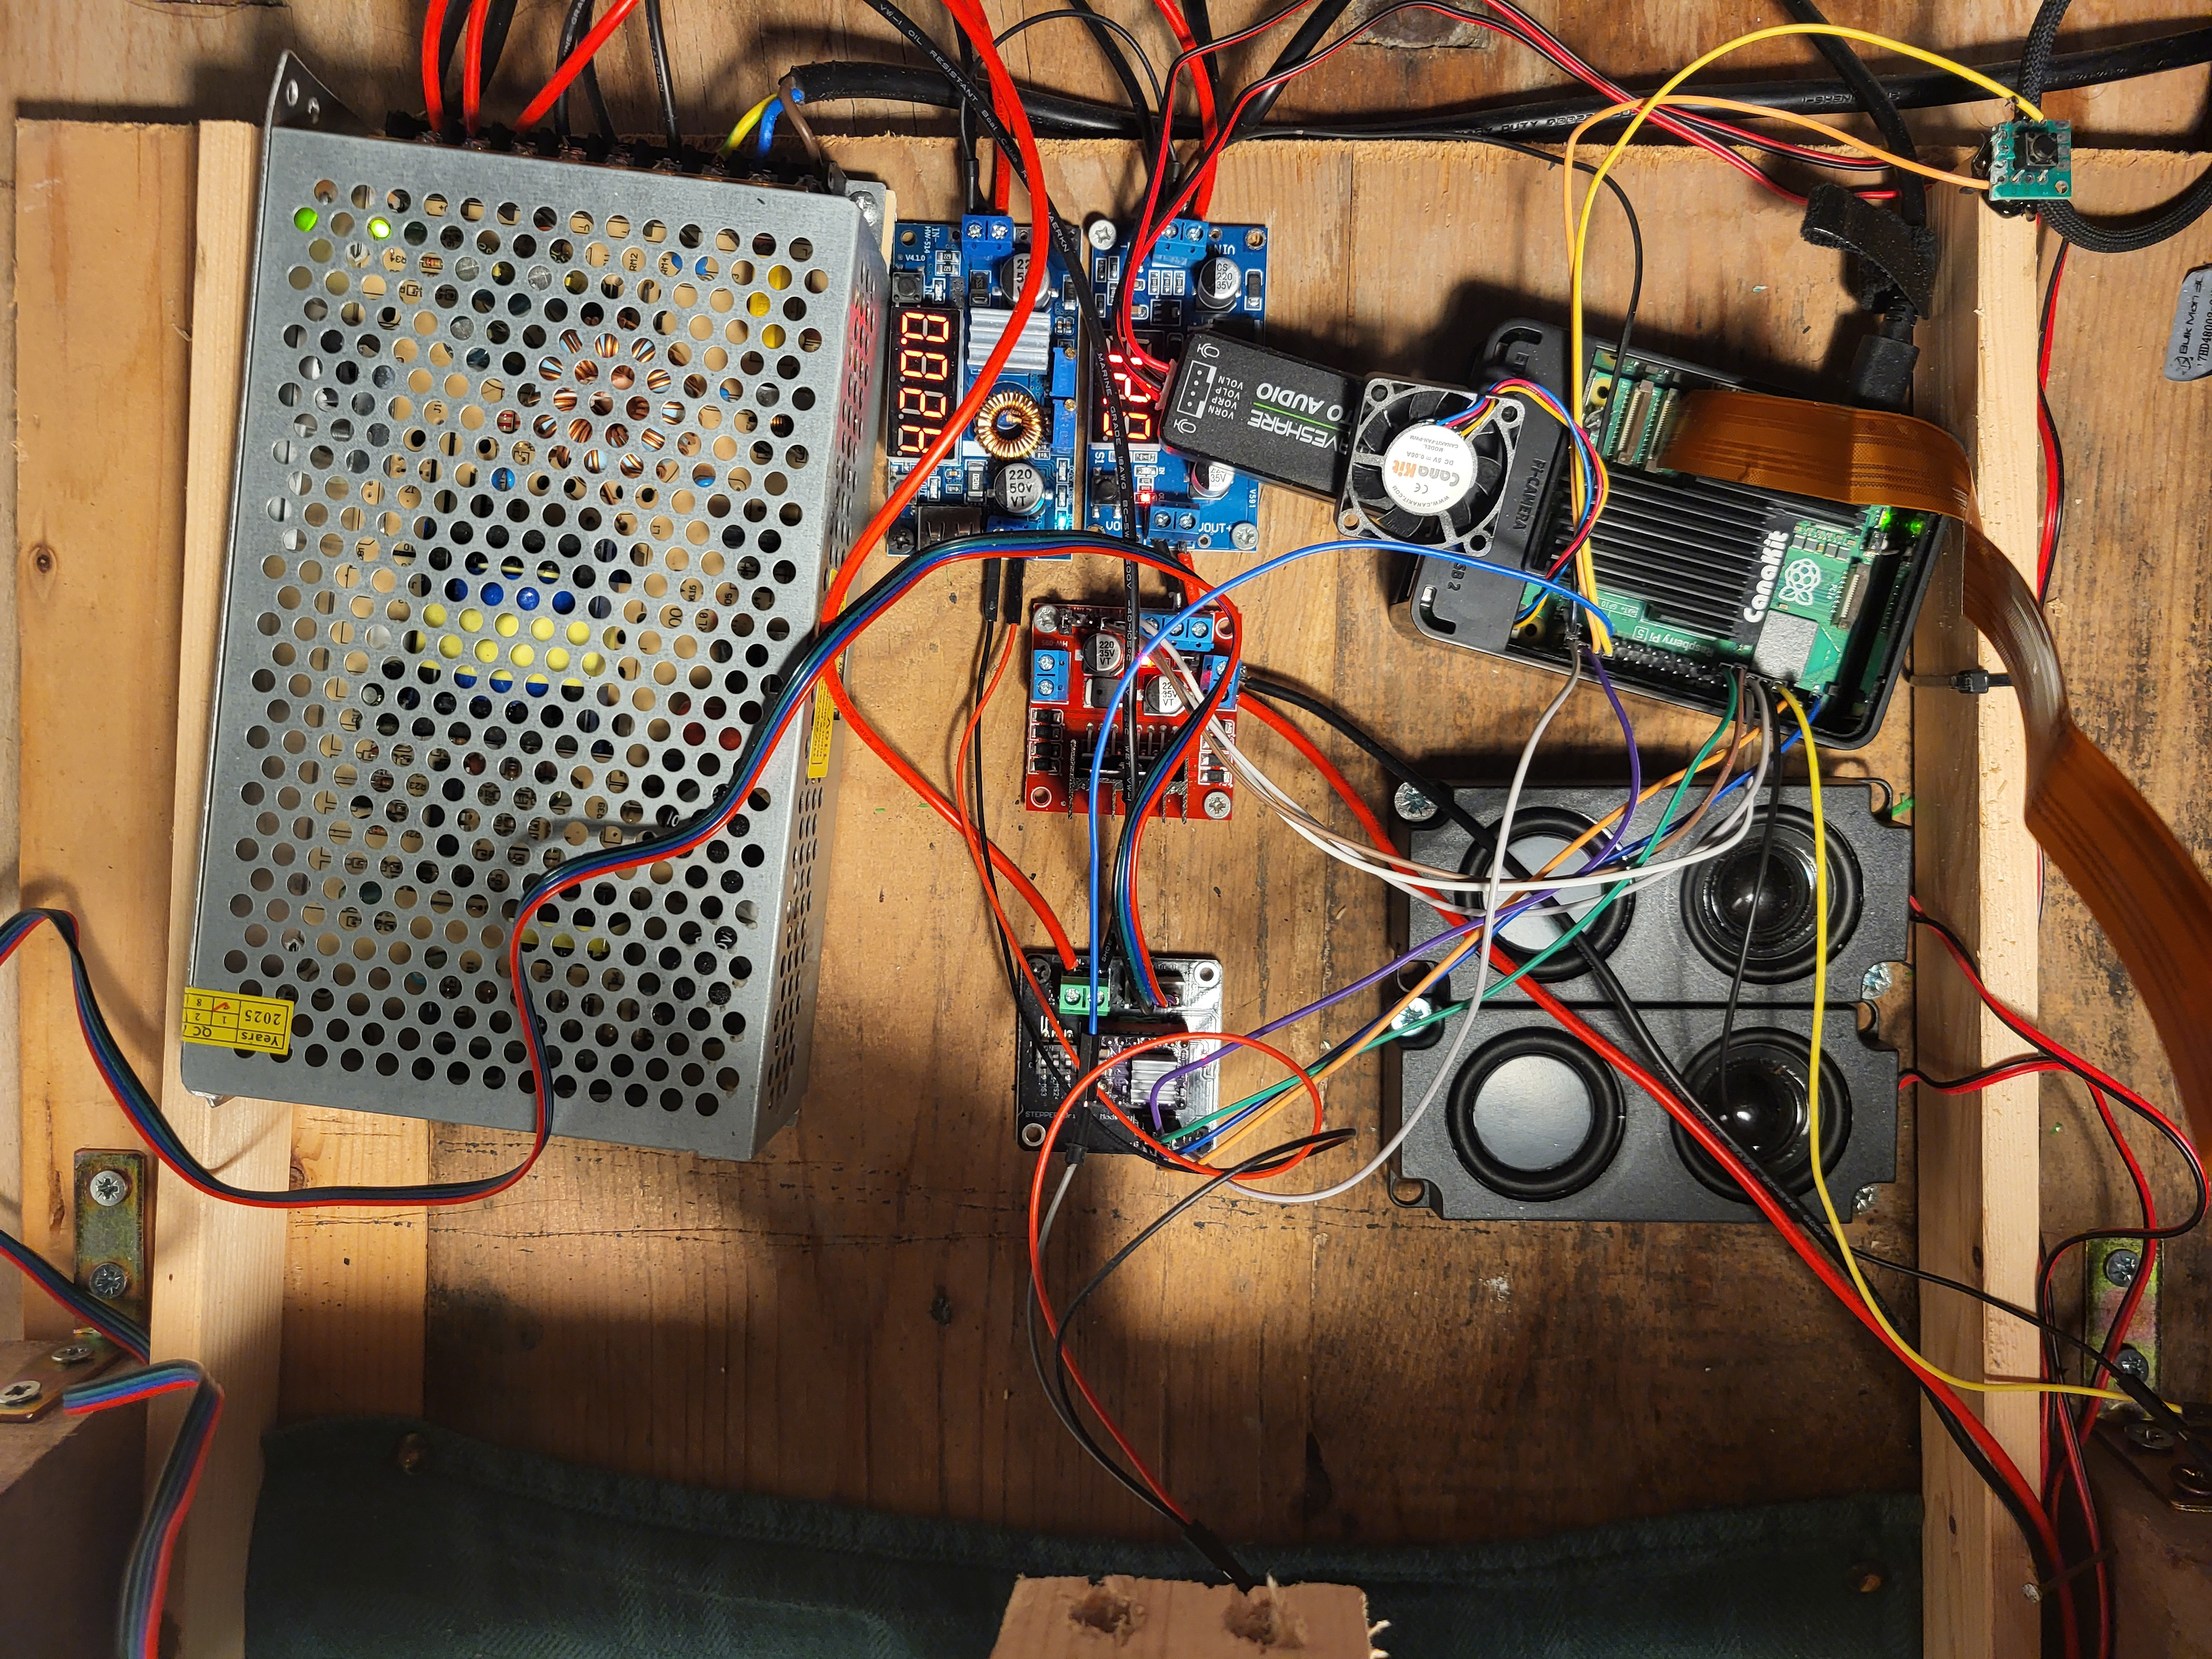
\includegraphics[angle=-90, width=0.49\textwidth]{../images/wiring_above.jpg}
    \includegraphics[angle=-90, width=0.49\textwidth]{../images/backend.jpg}
    \caption{Il setup elettronico: Raspberry Pi 5, drivers e convertitori.}
    \label{fig:electronics_photos}
\end{figure}
\newpage

\begin{figure}[H]
    \centering
    \includegraphics[width=\textwidth]{../images/blueprint.png}
    \caption{Schema elettrico del sistema (realizzato con EasyEDA). Mostra i collegamenti tra PSU, convertitori XL4015, driver (L298N, DRV8825) e Raspberry Pi.}
    \label{fig:blueprint}
\end{figure}

\subsection{Controller e Interfacce}
Il cervello è un \textbf{Raspberry Pi 5}.

Il limit switch e un pulsante fisico di controllo sono stati saldati ai loro fili e collegati direttamente ai pin GPIO. 
    
Il pulsante è stato fissato con colla a caldo a lato della piattaforma per facile accesso.

Non avendo il Pi 5 speaker integrati, sono stati aggiunti degli speaker USB esterni per permettere al robot di parlare.
\newpage

\section{Le Sfide dello Sviluppo (Problem Solving)}

\subsection{Il Servo: Problemi di Corrente}
Una delle difficoltà maggiori ha riguardato il motore di tiro. Inizialmente avevo scelto un servo da 15kg. Questo motore richiedeva picchi di corrente altissimi.
\begin{enumerate}
    \item Durante i test, è emerso che il servo operava in direzione opposta rispetto alla logica software, problema risolto invertendo i parametri di movimento nel codice.
    \item Il primo convertitore installato non ha retto il carico e si è fritto dopo qualche giorno di prove, ma questo è successo in parallelo con una vacanza che ho preso, non facendomi notare che fosse colpa del servo, e facendomelo sostituire senza grossi pensieri.
    \item Sostituito con un modello "premium" più costoso, quest'ultimo andava in protezione rifiutandosi di erogare la corrente di picco.
    \item Cercando di capire dove fosse il problema, ho addirittura comprato alcuni condensatori da 2200 uF per cercare di attutire i picchi.
    \item Forzando il convertitore a fornire l'amperaggio richiesto, il servo stesso si è surriscaldato, cortocircuitandosi internamente e fondendosi.
\end{enumerate}
La soluzione è stata passare a un servo più piccolo da 5kg. Sebbene anche molto più lento (riducendo la forza d'impatto), combinato con la superficie a basso attrito (tovaglia) e la pallina pesante, è riuscito a garantire tiri adeguati senza stressare l'elettronica.

\subsection{Visione e Problemi Hardware}
L'implementazione della visione artificiale non è stata una passeggiata. Il cavo flat fornito nella confezione della fotocamera non era compatibile con i nuovi connettori del Raspberry Pi 5, costringendo all'acquisto di un cavo specifico. 

La calibrazione è stata lunga e complessa. Per migliorare il riconoscimento, è stato necessario dipingere i bordi della struttura in legno (originariamente chiaro) di marrone scuro e la pallina di bianco puro, poiché i loghi neri originali frammentavano il rilevamento dell'algoritmo.
\newpage

\subsection{Incidenti di Percorso e Debugging}
L'inesperienza nel debugging elettronico ha portato a diversi incidenti:
\begin{itemize}
    \item \textbf{Cortocircuiti:} Un driver DRV8825 è stato distrutto da una scintilla causata dallo scivolamento dei puntali del multimetro tra VCC e GND. Un altro è stato danneggiato usando un cacciavite non adatto sulla vite di regolazione della corrente.
    \item \textbf{Pin PWM Bruciato:} Un pin del Raspberry Pi dedicato al PWM ha smesso di funzionare (probabilmente a causa di ritorni di corrente), costringendo a una modifica software per rimappare il segnale su un altro pin (GPIO 19).
    \item \textbf{Cablaggio Stepper:} I cavi del motore stepper erano etichettati in modo errato (fasi invertite rispetto a quanto richiesto dallo shield), richiedendo tentativi e ricablaggio manuale dei 4 fili.
\end{itemize}

\subsection{Ambiente di Sviluppo Ostile}
Il progetto è stato sviluppato in un garage esterno non riscaldato durante i mesi di ottobre, novembre e dicembre. Il freddo ha reso difficile lavorare per lunghi periodi.

Inoltre, la logistica è stata complessa:
\begin{itemize}
    \item \textbf{Connettività:} Il Raspberry Pi spesso non si connetteva all'hotspot del telefono. Non avendo un monitor in garage, era necessario staccare tutto, portare il Pi in casa, collegarlo a HDMI/Mouse/Tastiera per debuggare la rete, e tornare in garage.
    \item \textbf{Corruzione Software:} Uno spegnimento improvviso (togliendo l'alimentazione brutalmente) ha corrotto il filesystem della scheda SD. È stato necessario riflashare l'OS.
    
    Questo ha causato ulteriori problemi perché la nuova versione dell'OS non era identica a quella preinstallata, creando incompatibilità con le librerie Python precedentemente usate.
    \item \textbf{Alimentazione Pi:} Inizialmente, notando che il LED di stato del Raspberry si spegneva in boot, ho temuto fenomeni di "Brown-out" (tensione insufficiente). Ho quindi sostituito l'alimentatore originale (che era un modello USA con adattatore precario) con uno nuovo, pensando fosse la causa dei crash.
    
    Solo successivamente ho scoperto che i malfunzionamenti erano dovuti probabilmente alla corruzione dell'OS: essendo il sistema headless, non potevo vedere gli errori di boot e interpretavo lo spegnimento dei LED come un calo di tensione. Tuttavia, la sostituzione dell'alimentatore ha comunque migliorato la stabilità generale.
\end{itemize}

\section{Software: AI e Integrazione}
Dal punto di vista software, la sfida principale è stata l'integrazione delle librerie.
\textbf{Text-to-Speech:} La libreria standard \textit{eSpeak} aveva una qualità vocale terribile, troppo robotica. Ho scelto di passare a \textbf{Piper TTS}, che offre voci neurali molto realistiche. Tuttavia, installare e configurare Piper sul Raspberry Pi ha richiesto una gestione alquanto complessa di dipendenze e pacchetti.
\textbf{La buca:} Avere una buca fisica mobile era impratica. Si è scelto invece un chiodo con bandierina. Il software considera "buca" se la pallina colpisce il chiodo o/e si ferma entro una certa distanza.

\section{Conclusioni}
Costruire S.I.S.I.F.O. è stato un esercizio di perseveranza. Oltre alla programmazione, ha richiesto abilità di falegnameria, progettazione elettrica e una notevole dose di problem-solving pratico. 

I malfunzionamenti hardware e le condizioni hanno trasformato un progetto teorico in una reale esperienza ingegneristica, dove far coesistere pezzi di legno di recupero con le più recenti tecnologie di Intelligenza Artificiale, ma soprattutto l'aver vinto una battaglia contro l'elettronica è stata la vera vittoria.

Se ci sono due cose che ho imparato da questo progetto, è l'indomabile spirito umano, e quanto si sta bene al caldo a programmare digitalmente invece di fisicamente.

\end{document}
